\chapter{ Констукторский раздел}
\label{cha:design}
    В данном разделе будут рассмотрены схемы алгоритмов, требования к функциональности ПО,
    и опредены способы тестирования.
    
    \section{Разработка алгоритмов}
        Ниже будут представлены схемы алгоритмов умножения матриц: \begin{enumerate}
            \item классического (рисунок \ref{schema:standartDot});
            \item Винограда (рисунок \ref{schema:vinogradDot});
            \item оптимизированного Винограда (рисунок \ref{schema:vinogradDot:optimize}).
        \end{enumerate}

    Для уменьшения трудоёмкости алгоритма Винограда сделаем следующие действия:
    \begin{enumerate}
        \item замена в цикле условии деления на 2 на цикл с шагом 2
        \item замена a = a + ..., на a += ...
        \item вычисление суммы отрицательной при заполнении row и col 
    \end{enumerate}

\section{Оценка трудоёмкости алгоритмов умножения матриц}

  \subsection{Стандартный алгоритм}
            Найдём трудоёмкость стандартного алгоритма.
            
            $ f_\text{первый цикл} = 2 + M(2 + f_\text{второй цикл})$  

            $ f_\text{второй цикл} = 2 + Q(2 + f_\text{третий цикл})$  

            $ f_\text{третий цикл} = 2 + N(2 + 11)$  

            $ f_\text{Стандартный} = 13MNQ + 4MQ + 4M + 2 \approx 13MNQ$

        \subsection{Алгоритм Винограда}
            Найдём трудоёмкость алгоритма Винограда.
            
            $ f_\text{первый цикл} = 2 + M(2 + 2 + 3 + \frac{N}{2}(3 + 1 + 6 + 2 + 3)) = \frac{15}{2}MN + 7M + 2$
            
            $ f_\text{второй цикл} = \frac{15}{2}QN + 7Q + 2$

            $ f_\text{третий цикл} = 2 + M(2 + 2 + Q(2 + 7 + 3 + \frac{N}{2}(3 + 1 + 12 + 5 + 5))) = 13MNQ + 12MQ + 4M + 2$

            Условный переход $f_{if} = 2 + \left\{
                \begin{matrix}
                0 - \text{лучший случай},\\
                15QM + 4M + 2 - \text{худший случай} 
                \end{matrix}\right.$

            Итого:
            \begin{equation}
                f_\text{Винограда} = 13MNQ + 12MQ + \frac{15}{2}(MN + QN) + 7(M + Q) + 4M + 8 + 
                    \left\{ \begin{matrix}
                    0 - \text{л.с.},\\
                    15MQ + 4M + 2 - \text{х.с.} 
                    \end{matrix}\right.
            \end{equation}
            $ f_\text{Винограда} \approx 13MNQ $
        \subsection{Оптимизированный алгоритм Винограда}

            Найдём трудоёмкость оптимизированного алгоритма Винограда.
                
            $ f_\text{первый цикл}^* = 2 + M(2 + 2 + 2 + \frac{N}{2}(2 + 1 + 5 + 1 + 1)) = 10MN + 6M + 2$
            
            $ f_\text{второй цикл}^* = 10MN + 6M + 2$

            $ f_\text{третий цикл}^* = 2 + M(2 + 2 + Q(2 + 6 + 2 + \frac{N}{2}(2 + 1 + 10 + 4 + 1))) = 9MNQ + 10MQ + 4M + 2$

            Условный переход $f_{if}^* = 2 + \left\{
                \begin{matrix}
                0 - \text{лучший случай},\\
                12QM + 4M + 2 - \text{худший случай} 
                \end{matrix}\right.$

            Итого:
            \begin{equation}
                f_\text{Винограда}^* = 9MNQ + 10MQ + \frac{15}{2}(MN + QN) + 6(M + Q) + 4M + 8 + 
                    \left\{ \begin{matrix}
                    0 - \text{л.с.},\\
                    12MQ + 4M + 2 - \text{х.с.} 
                    \end{matrix}\right.
            \end{equation}
            $ f_\text{Винограда}^* \approx 9MNQ $

    \section{Вывод}
       При одинаковом коэффициенте при старшем слагаемом в трудоемкости алгоритма Винограда и стандартного, доля долгих операций умножения в алгоритме Винограда меньше.
        Стоит отметить, что алгоритм Винограда имеет худший (матрицы совпадающей нечётной размерности -- количество строк матрицы А и столбцов матрицы В) и лучший случаи (матрицы совпадающей чётной размерности -- количество строк матрицы А и столбцов матрицы В),
        в то время как стандартный алгоритм не зависит от чётности совпадающей размерности матриц. Путем оптимизации трудоемкость алгоритма Винограда была снижена.


    \begin{figure}[h!]
        \centering
            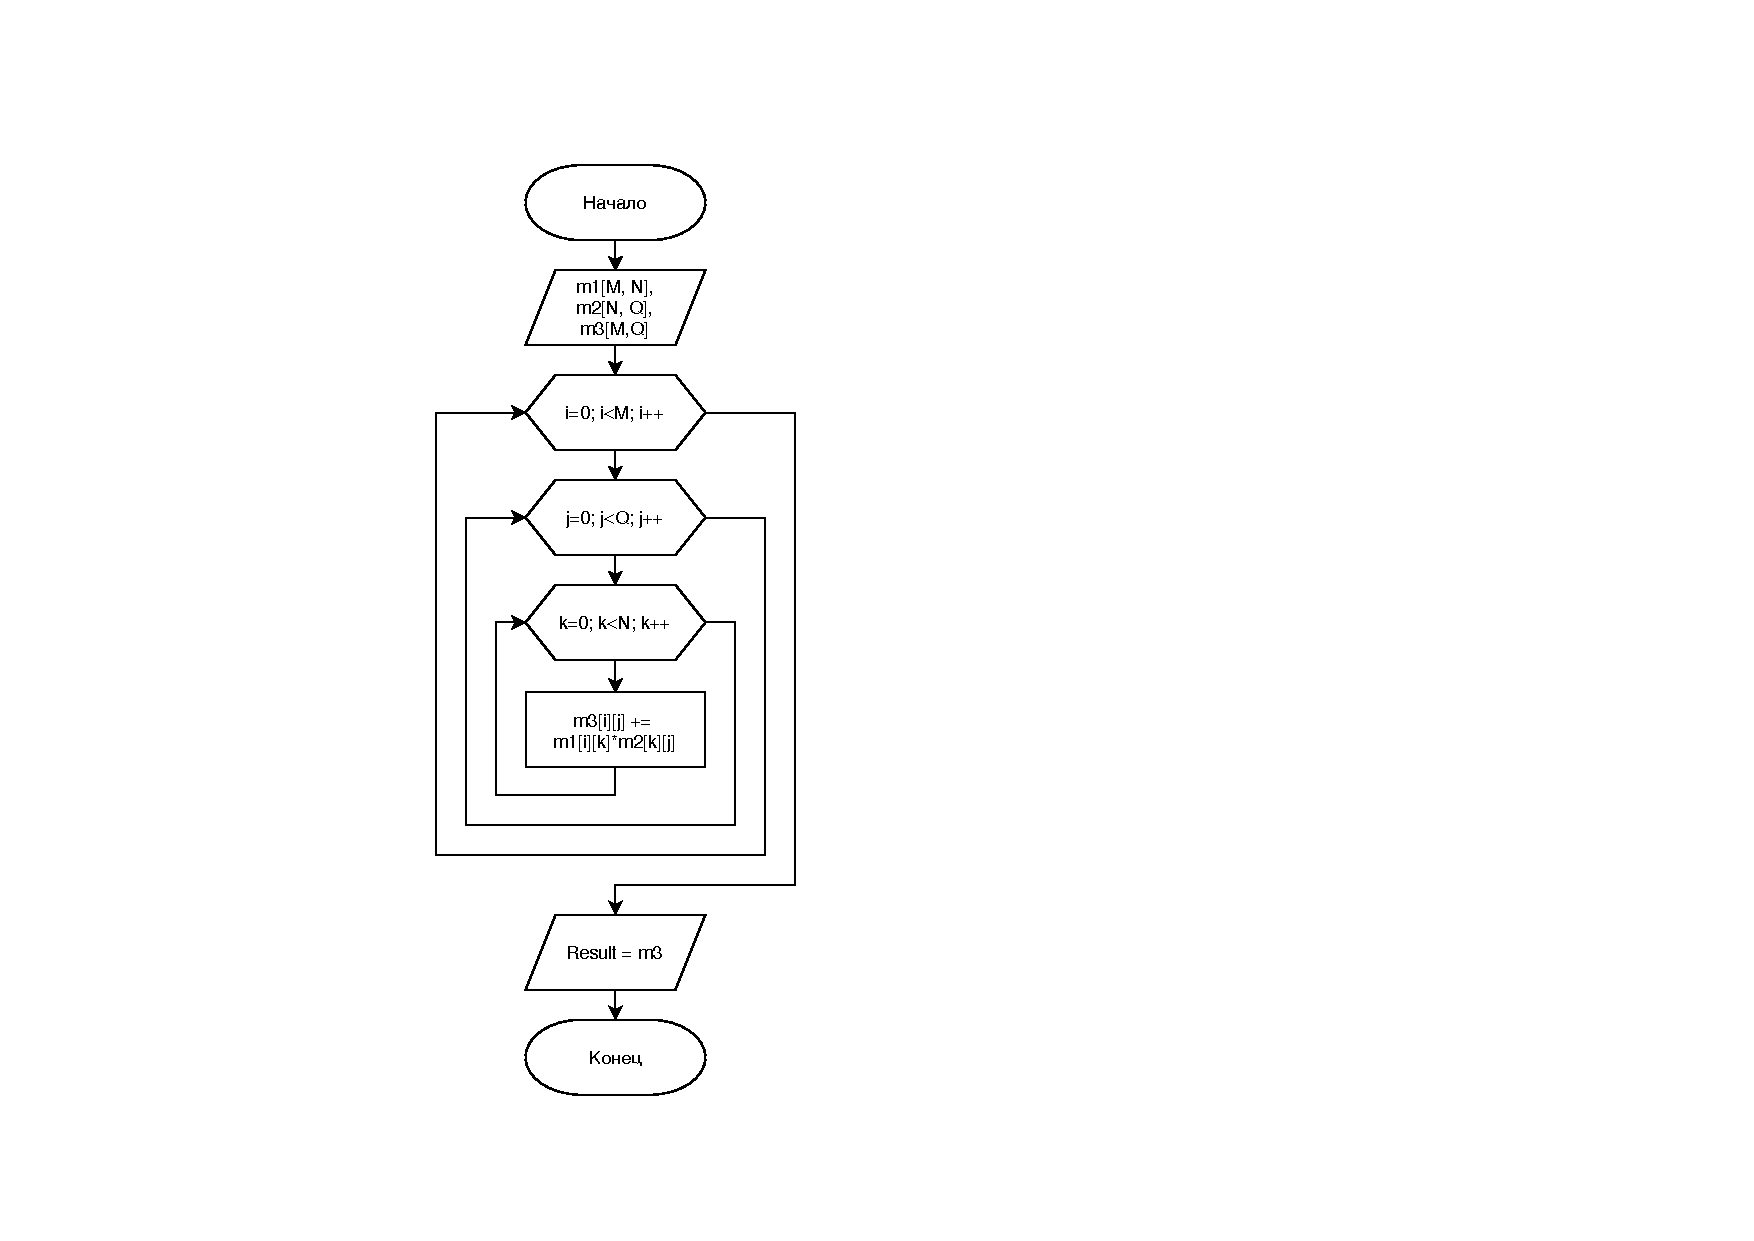
\includegraphics[scale=0.9]{schema_std.pdf}
            \caption{Схема стандартного алгоритма умножения матриц}
            \label{schema:standartDot}
    \end{figure}

    \begin{figure}[h!]
        \centering
            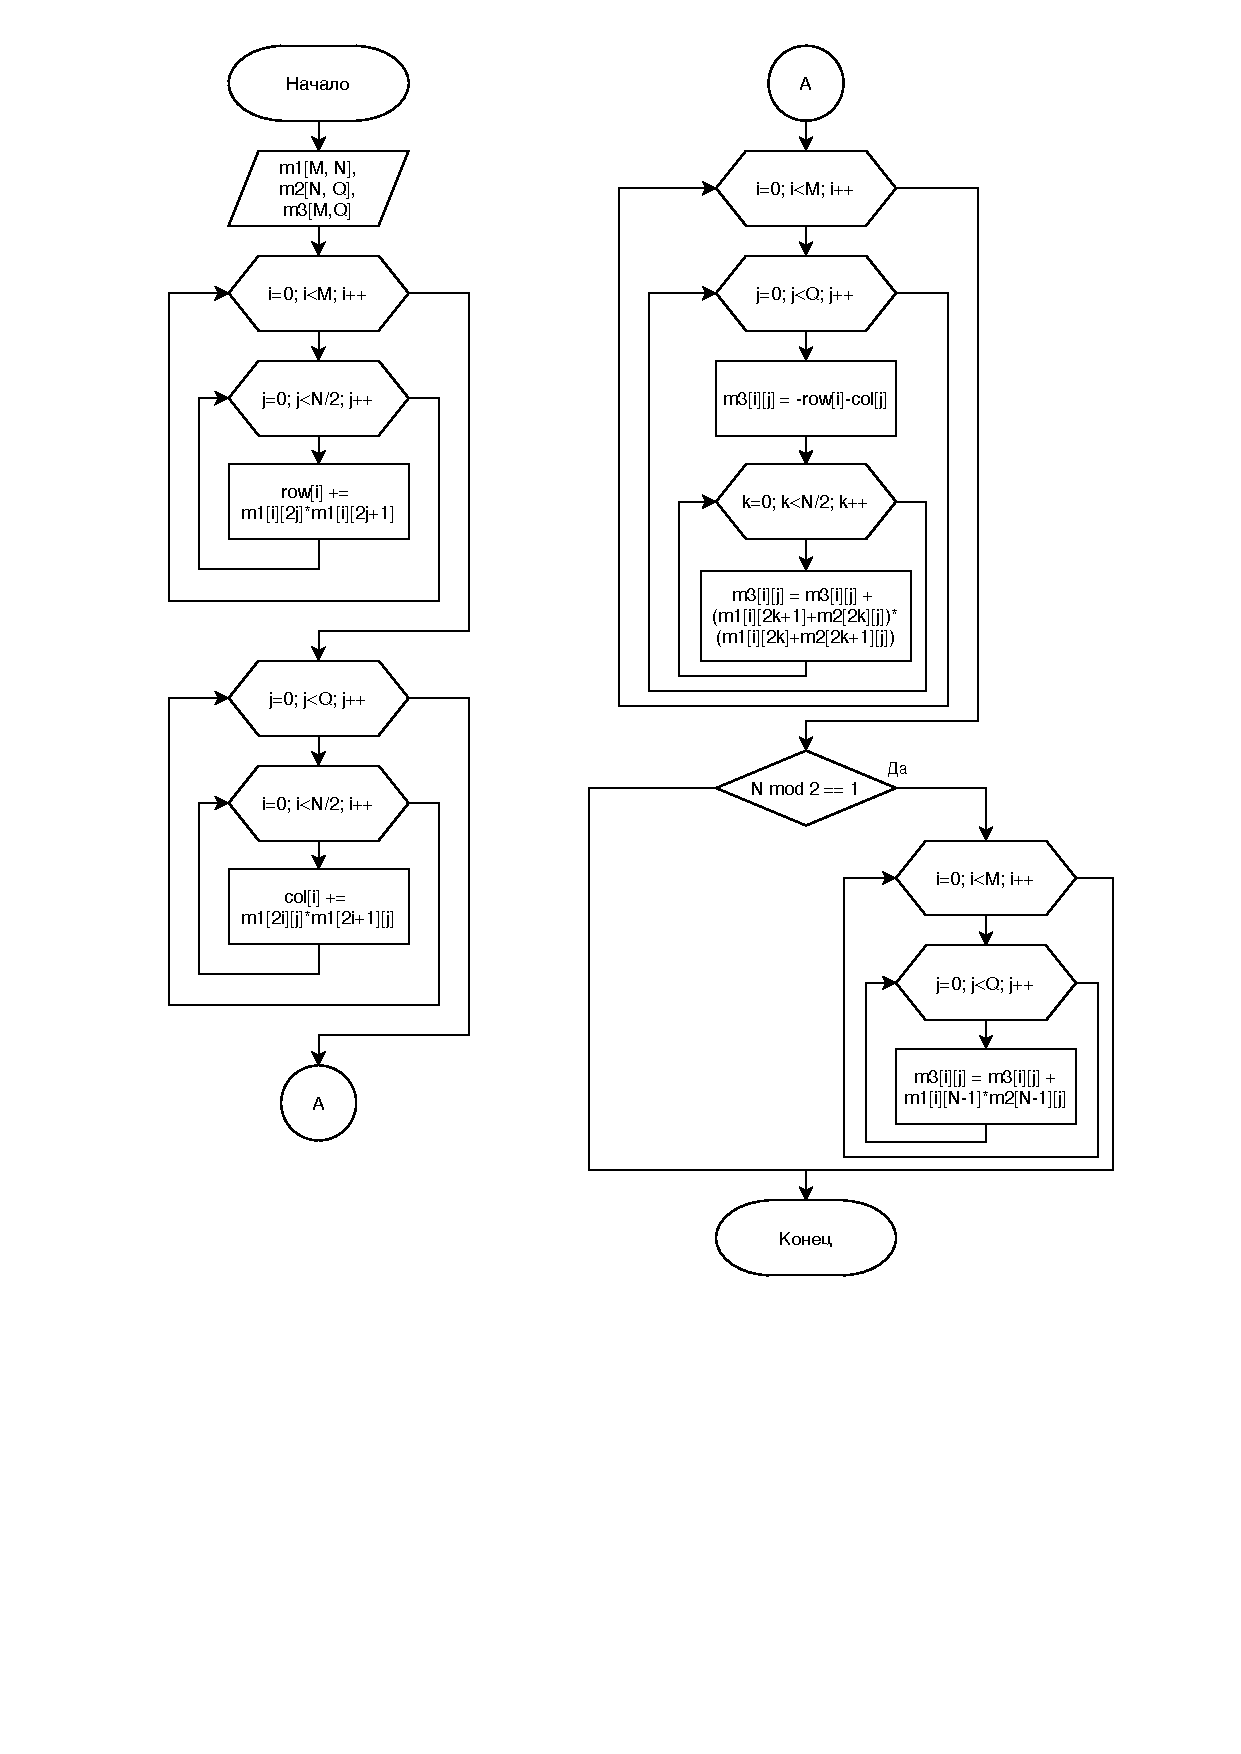
\includegraphics[scale=0.9]{schema_vin.pdf}
            \caption{Схема алгоритма умножения матриц методом Винограда}
            \label{schema:vinogradDot}
    \end{figure}

    \begin{figure}[h!]
        \centering
            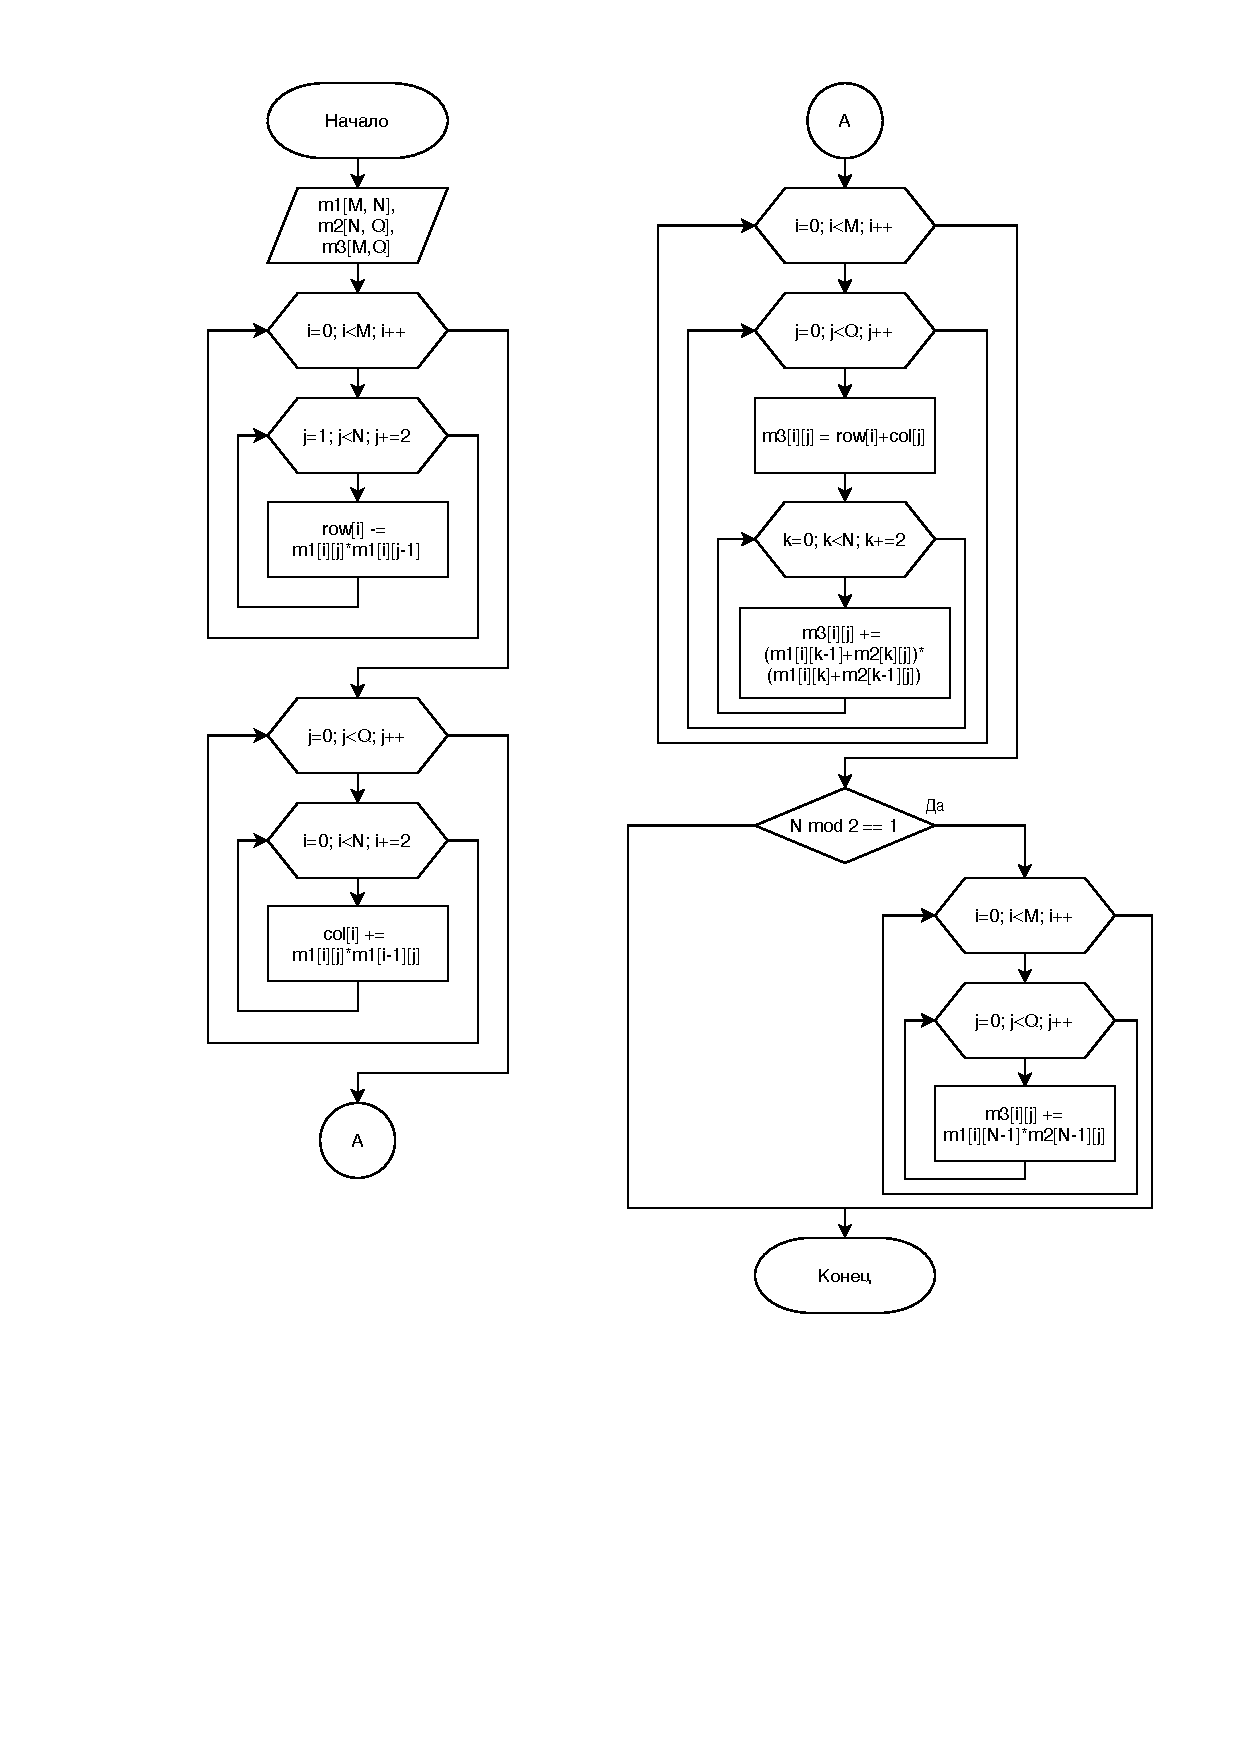
\includegraphics[scale=0.9]{schema_vinOpt.pdf}
            \caption{Схема оптимизированный алгоритм умножения матриц методом Винограда}
            \label{schema:vinogradDot:optimize}
    \end{figure}

    \section{Требования к функциональности ПО}
        В данной работе требуется обеспечить следующую минимальную функциональность консольного приложения:
        \begin{enumerate}
            \item возможность ввода двух матриц, на выходе результат произведения данных матриц, посчитанный трёмя алгоритмами;
            \item возможность вывода результатов замера процессорного времени работы реализаций каждого из алгоритмов. 
        \end{enumerate}

    \section{Требования к тестированию}
    Тестирование ПО будет проводиться методом чёрного ящика. Необходимо проверить работу системы 
    на тривиальных случаях (одна матрица единичная или нулевая) 
    и несколько нетривальных случаев.

\newpage